% !TEX root = ../../main.tex

\section{Calorimetry MIL-100(Fe)}

\begin{figure}[H]
    \centering

    \begin{subfigure}{0.25\linewidth}
        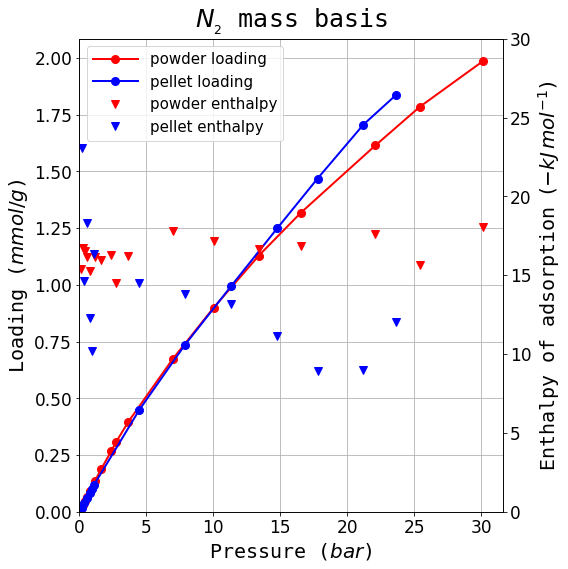
\includegraphics[width=\textwidth]{calo/MIL-100(Fe)/nitrogen-mass-basis-iso}%
        \label{appx:fig:shaping:mil100n2mass}
    \end{subfigure}%
    \begin{subfigure}{0.25\linewidth}
        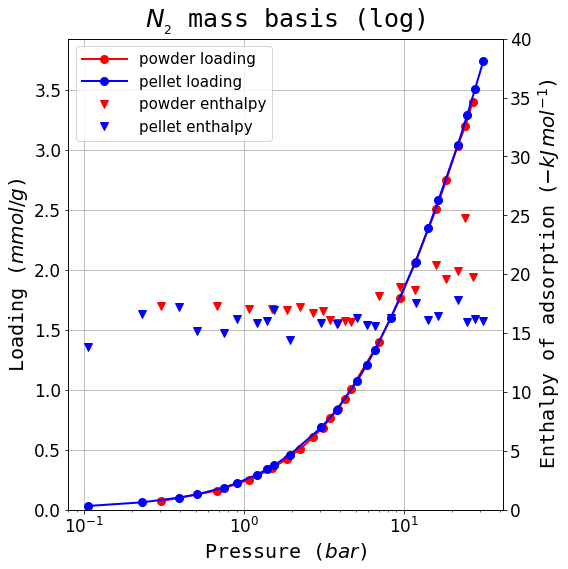
\includegraphics[width=\textwidth]{calo/MIL-100(Fe)/nitrogen-mass-basis-log-iso}%
        \label{appx:fig:shaping:mil100n2masslog}
    \end{subfigure}%
    \begin{subfigure}{0.25\linewidth}
        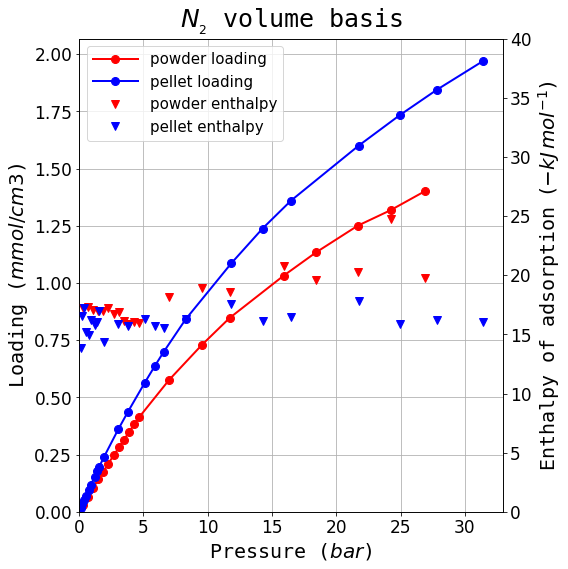
\includegraphics[width=\textwidth]{calo/MIL-100(Fe)/nitrogen-volume-basis-iso}%
        \label{appx:fig:shaping:mil100n2volume}
    \end{subfigure}%
    \begin{subfigure}{0.25\linewidth}
        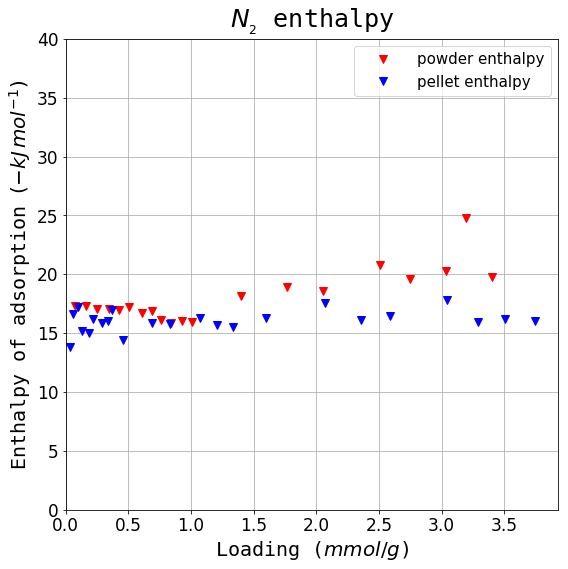
\includegraphics[width=\textwidth]{calo/MIL-100(Fe)/nitrogen-enth}%
        \label{appx:fig:shaping:mil100n2enth}
    \end{subfigure}%
    
    \begin{subfigure}{0.25\textwidth}
        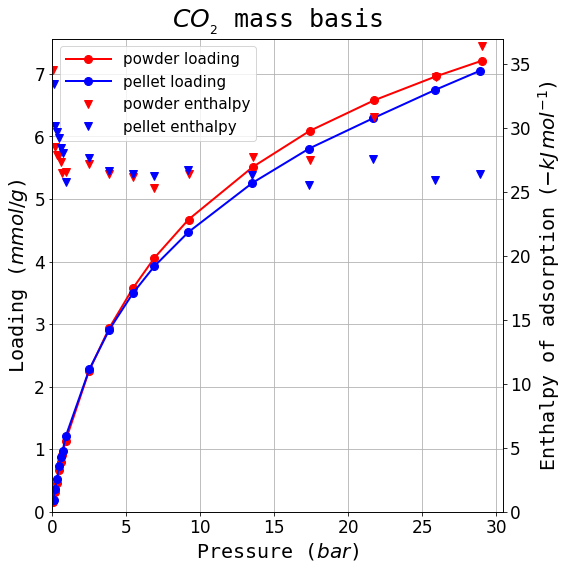
\includegraphics[width=\textwidth]{calo/MIL-100(Fe)/carbondioxide-mass-basis-iso}%
        \label{appx:fig:shaping:mil100co2mass}
    \end{subfigure}%
    \begin{subfigure}{0.25\textwidth}
        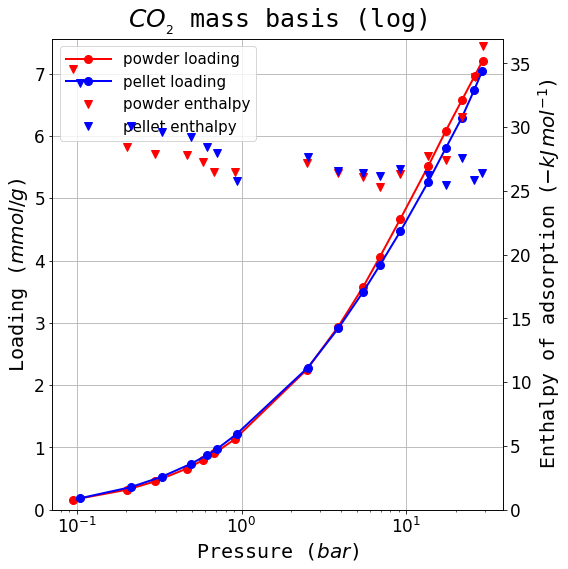
\includegraphics[width=\textwidth]{calo/MIL-100(Fe)/carbondioxide-mass-basis-log-iso}%
        \label{appx:fig:shaping:mil100co2masslog}
    \end{subfigure}%
    \begin{subfigure}{0.25\textwidth}
        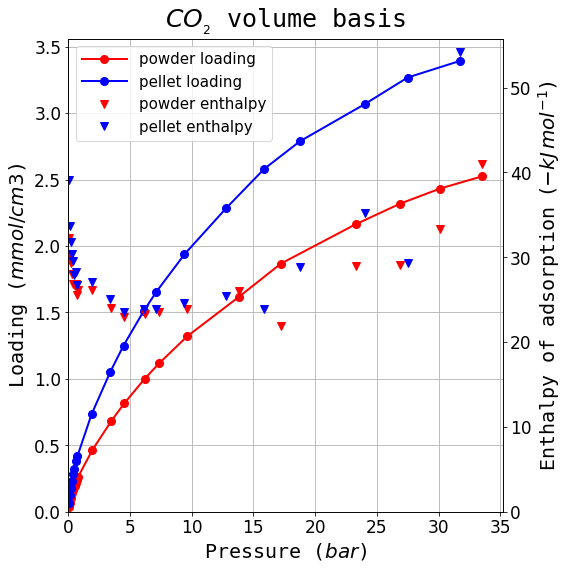
\includegraphics[width=\textwidth]{calo/MIL-100(Fe)/carbondioxide-volume-basis-iso}%
        \label{appx:fig:shaping:mil100co2volume}
    \end{subfigure}%
    \begin{subfigure}{0.25\textwidth}
        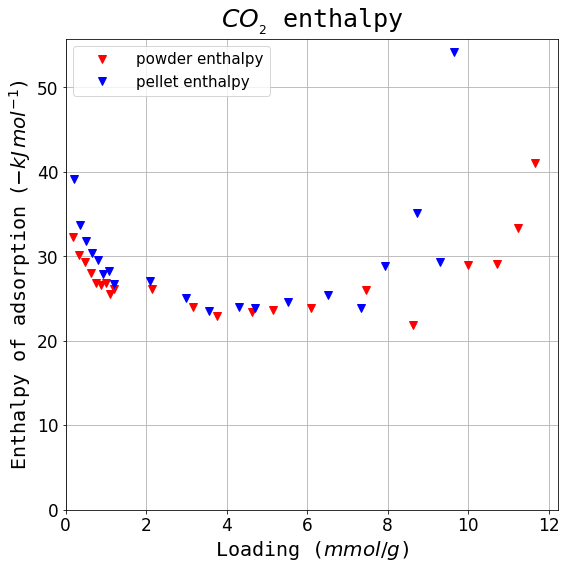
\includegraphics[width=\textwidth]{calo/MIL-100(Fe)/carbondioxide-enth}%
        \label{appx:fig:shaping:mil100co2enth}
    \end{subfigure}%

    \begin{subfigure}{0.25\textwidth}
        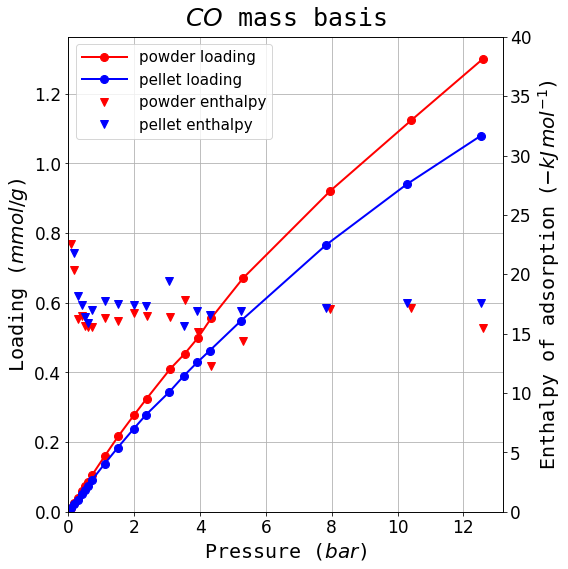
\includegraphics[width=\textwidth]{calo/MIL-100(Fe)/carbonmonoxide-mass-basis-iso}%
        \label{appx:fig:shaping:mil100comass}
    \end{subfigure}%
    \begin{subfigure}{0.25\textwidth}
        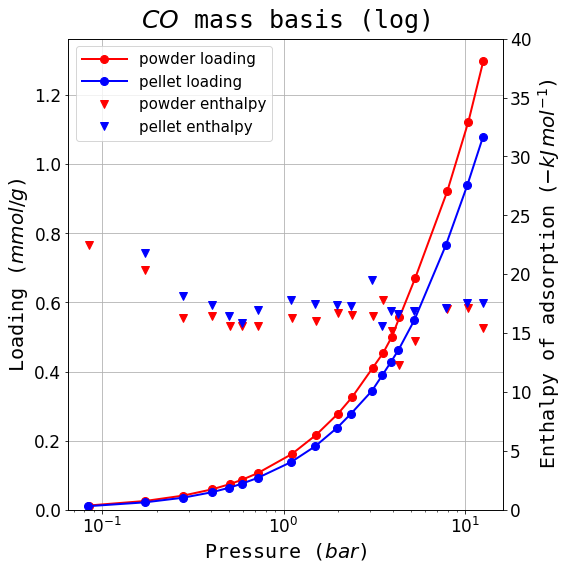
\includegraphics[width=\textwidth]{calo/MIL-100(Fe)/carbonmonoxide-mass-basis-log-iso}%
        \label{appx:fig:shaping:mil100comasslog}
    \end{subfigure}%
    \begin{subfigure}{0.25\textwidth}
        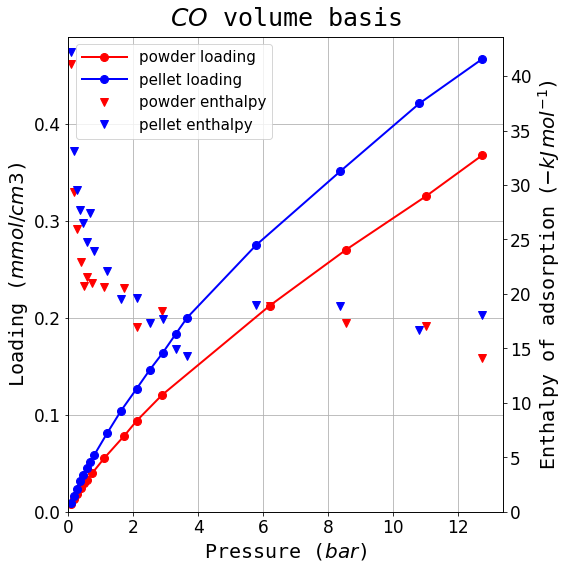
\includegraphics[width=\textwidth]{calo/MIL-100(Fe)/carbonmonoxide-volume-basis-iso}%
        \label{appx:fig:shaping:mil100covolume}
    \end{subfigure}%
    \begin{subfigure}{0.25\textwidth}
        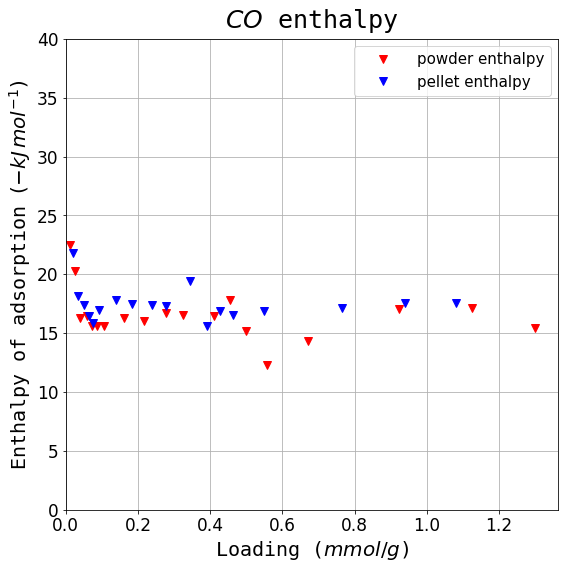
\includegraphics[width=\textwidth]{calo/MIL-100(Fe)/carbonmonoxide-enth}%
        \label{appx:fig:shaping:mil100coenth}
    \end{subfigure}%


    \begin{subfigure}{0.25\textwidth}
        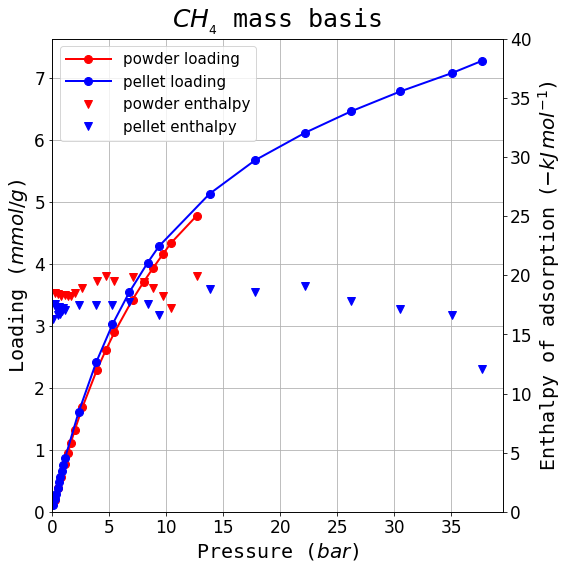
\includegraphics[width=\textwidth]{calo/MIL-100(Fe)/methane-mass-basis-iso}%
        \label{appx:fig:shaping:mil100ch4mass}
    \end{subfigure}%
    \begin{subfigure}{0.25\textwidth}
        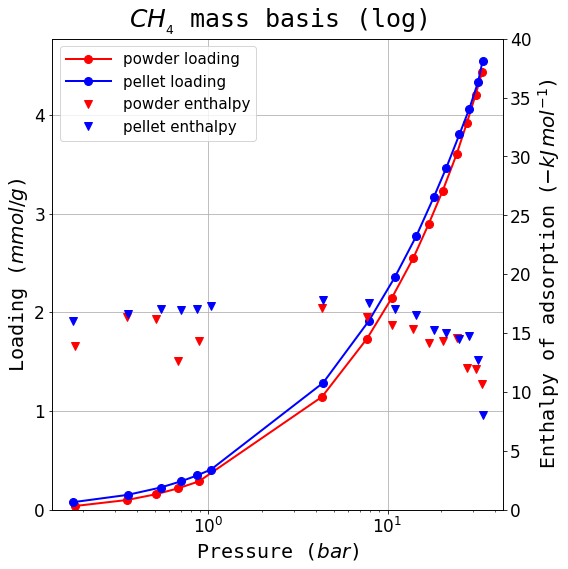
\includegraphics[width=\textwidth]{calo/MIL-100(Fe)/methane-mass-basis-log-iso}%
        \label{appx:fig:shaping:mil100ch4masslog}
    \end{subfigure}%
    \begin{subfigure}{0.25\textwidth}
        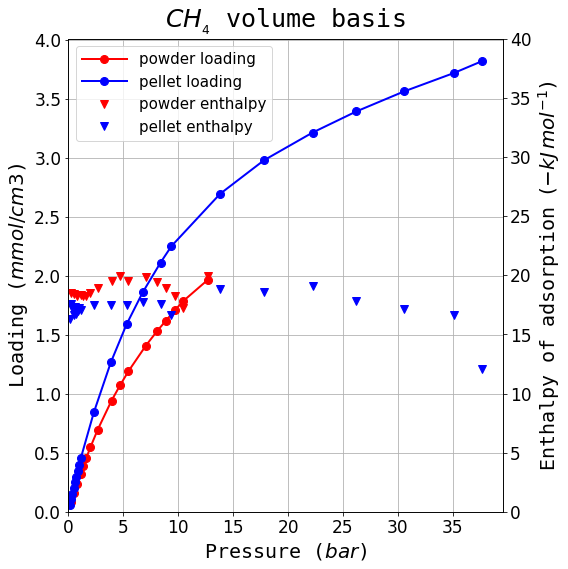
\includegraphics[width=\textwidth]{calo/MIL-100(Fe)/methane-volume-basis-iso}%
        \label{appx:fig:shaping:mil100ch4volume}
    \end{subfigure}%
    \begin{subfigure}{0.25\textwidth}
        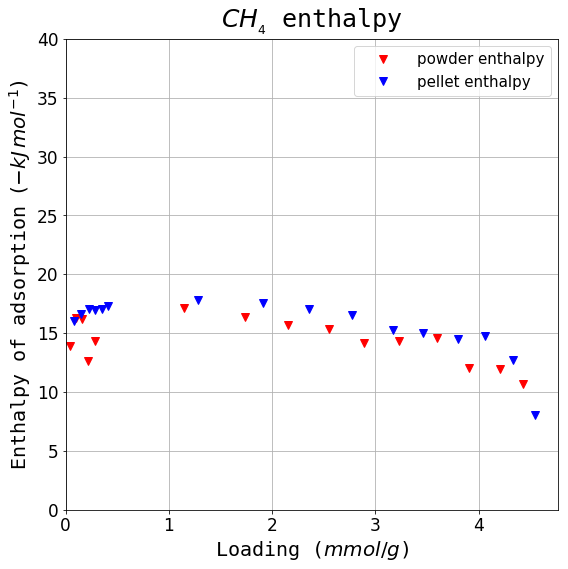
\includegraphics[width=\textwidth]{calo/MIL-100(Fe)/methane-enth}%
        \label{appx:fig:shaping:mil100ch4enth}
    \end{subfigure}%

    \caption{Complete isotherm and enthalpy dataset for MIL-100(Fe)}
    
\end{figure}

\begin{figure}[H]

    \begin{subfigure}{0.25\textwidth}
        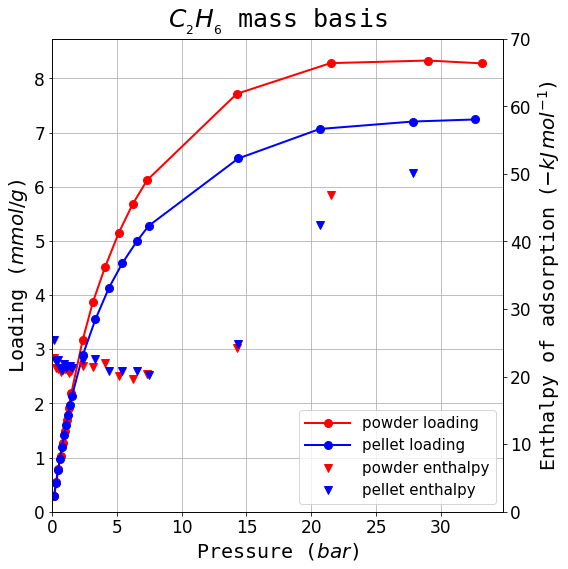
\includegraphics[width=\textwidth]{calo/MIL-100(Fe)/ethane-mass-basis-iso}%
        \label{appx:fig:shaping:mil100c2h6mass}
    \end{subfigure}%
    \begin{subfigure}{0.25\textwidth}
        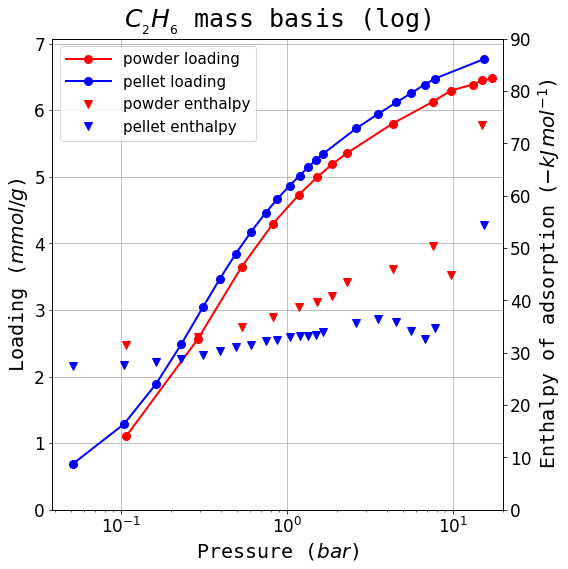
\includegraphics[width=\textwidth]{calo/MIL-100(Fe)/ethane-mass-basis-log-iso}%
        \label{appx:fig:shaping:mil100c2h6masslog}
    \end{subfigure}%
    \begin{subfigure}{0.25\textwidth}
        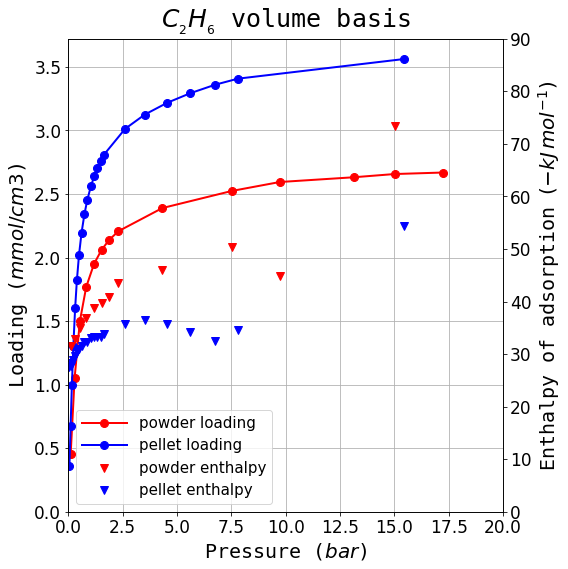
\includegraphics[width=\textwidth]{calo/MIL-100(Fe)/ethane-volume-basis-iso}%
        \label{appx:fig:shaping:mil100c2h6volume}
    \end{subfigure}%
    \begin{subfigure}{0.25\textwidth}
        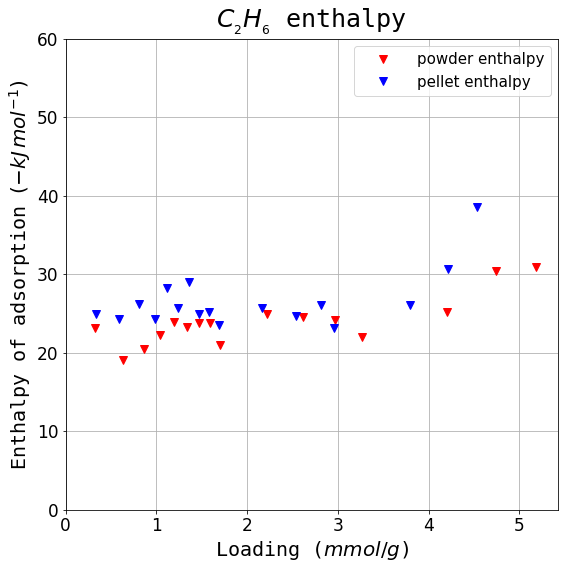
\includegraphics[width=\textwidth]{calo/MIL-100(Fe)/ethane-enth}%
        \label{appx:fig:shaping:mil100c2h6enth}
    \end{subfigure}%

    \begin{subfigure}{0.25\textwidth}
        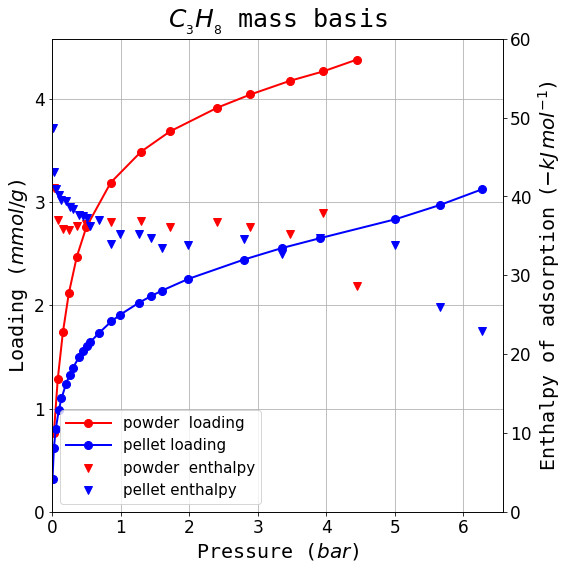
\includegraphics[width=\textwidth]{calo/MIL-100(Fe)/propane-mass-basis-iso}%
        \label{appx:fig:shaping:mil100c3h8mass}
    \end{subfigure}%
    \begin{subfigure}{0.25\textwidth}
        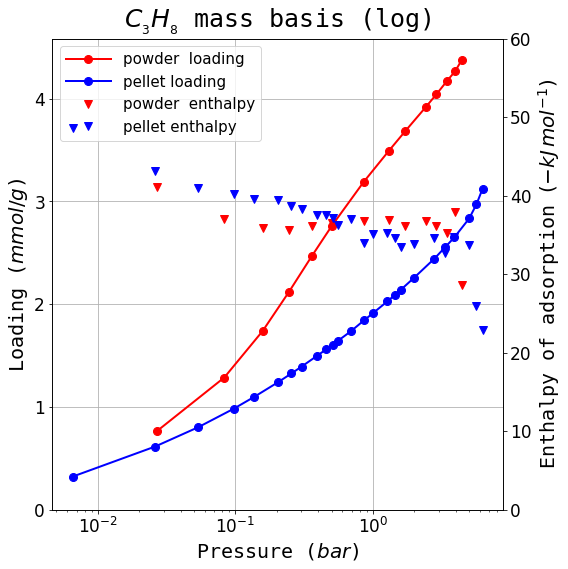
\includegraphics[width=\textwidth]{calo/MIL-100(Fe)/propane-mass-basis-log-iso}%
        \label{appx:fig:shaping:mil100c3h8masslog}
    \end{subfigure}%
    \begin{subfigure}{0.25\textwidth}
        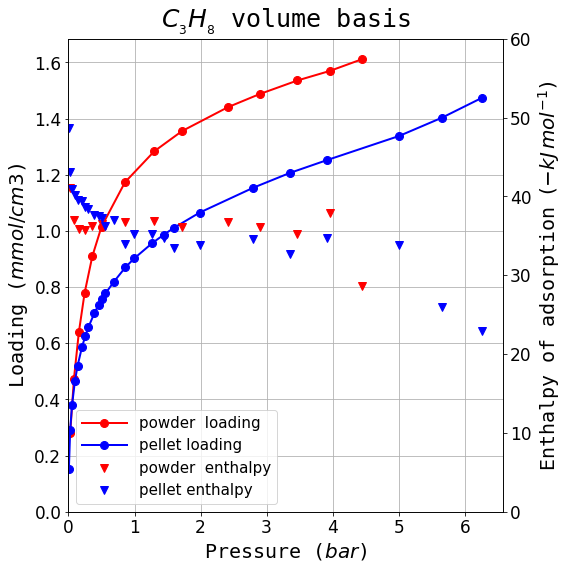
\includegraphics[width=\textwidth]{calo/MIL-100(Fe)/propane-volume-basis-iso}%
        \label{appx:fig:shaping:mil100c3h8volume}
    \end{subfigure}%
    \begin{subfigure}{0.25\textwidth}
        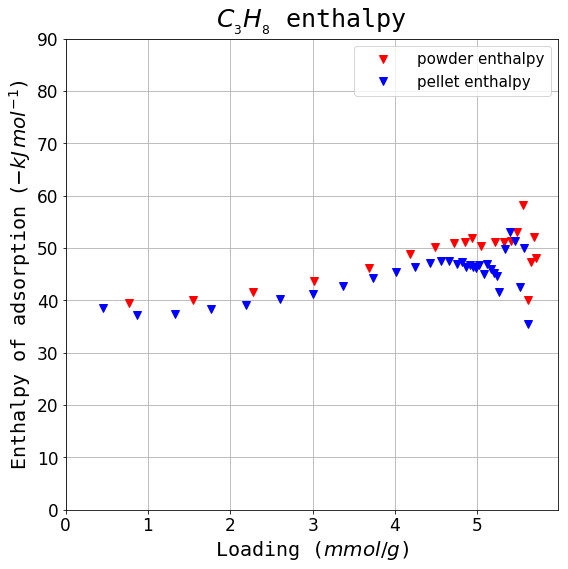
\includegraphics[width=\textwidth]{calo/MIL-100(Fe)/propane-enth}%
        \label{appx:fig:shaping:mil100c3h8enth}
    \end{subfigure}%

    \begin{subfigure}{0.25\textwidth}
        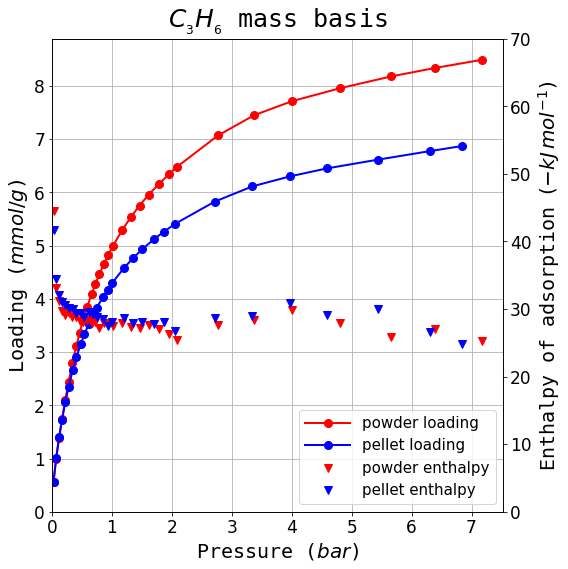
\includegraphics[width=\textwidth]{calo/MIL-100(Fe)/propene-mass-basis-iso}%
        \label{appx:fig:shaping:mil100c3h6mass}
    \end{subfigure}%
    \begin{subfigure}{0.25\textwidth}
        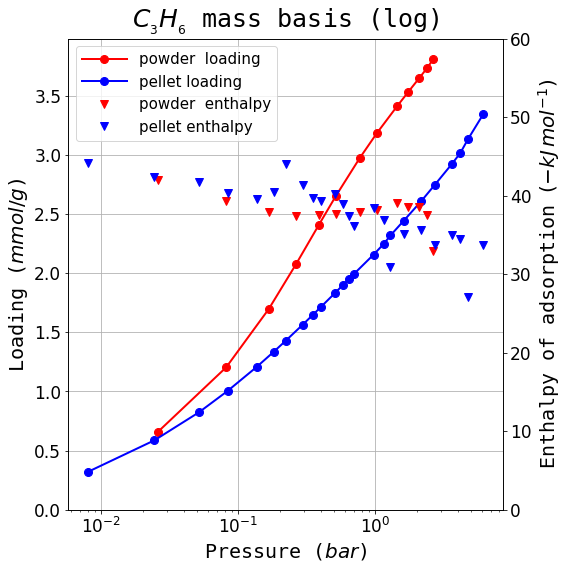
\includegraphics[width=\textwidth]{calo/MIL-100(Fe)/propene-mass-basis-log-iso}%
        \label{appx:fig:shaping:mil100c3h6masslog}
    \end{subfigure}%
    \begin{subfigure}{0.25\textwidth}
        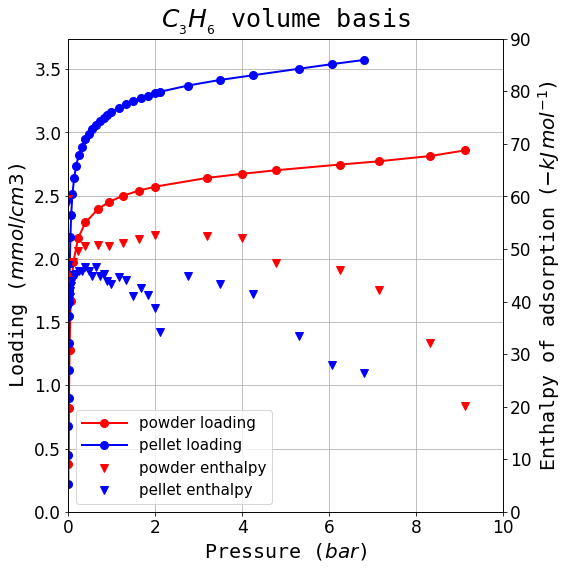
\includegraphics[width=\textwidth]{calo/MIL-100(Fe)/propene-volume-basis-iso}%
        \label{appx:fig:shaping:mil100c3h6volume}
    \end{subfigure}%
    \begin{subfigure}{0.25\textwidth}
        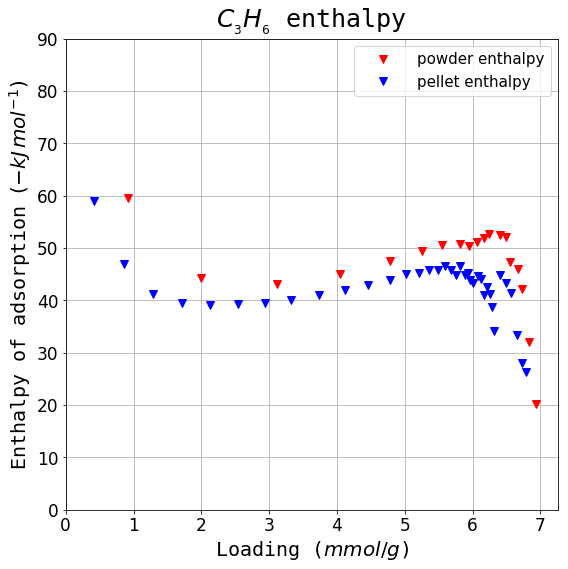
\includegraphics[width=\textwidth]{calo/MIL-100(Fe)/propene-enth}%
        \label{appx:fig:shaping:mil100c3h6enth}
    \end{subfigure}%

    \begin{subfigure}{0.25\textwidth}
        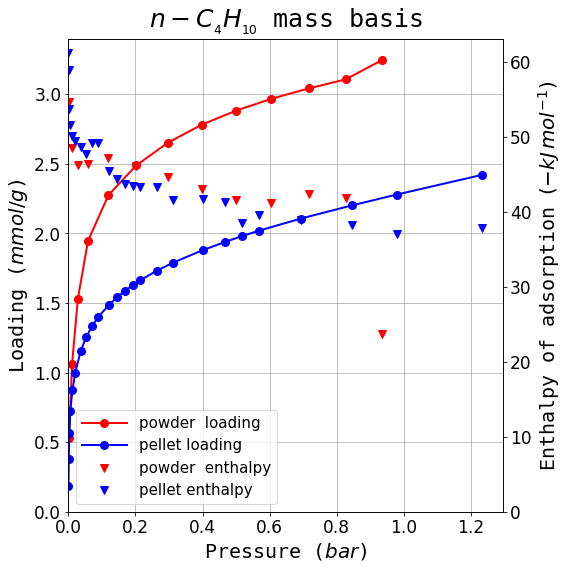
\includegraphics[width=\textwidth]{calo/MIL-100(Fe)/butane-mass-basis-iso}%
        \label{appx:fig:shaping:mil100c4h10mass}
    \end{subfigure}%
    \begin{subfigure}{0.25\textwidth}
        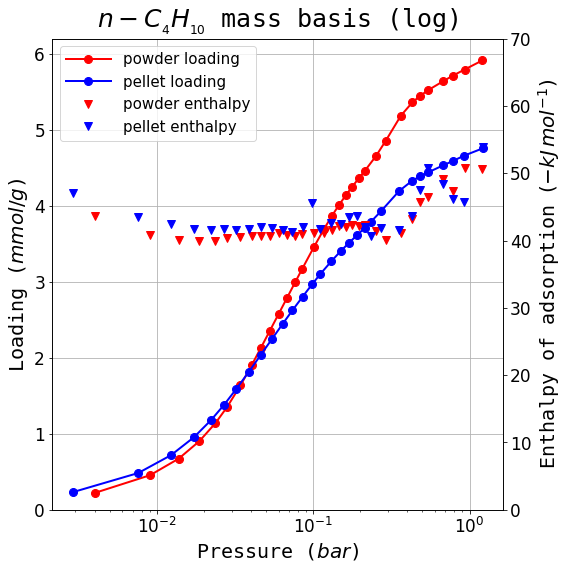
\includegraphics[width=\textwidth]{calo/MIL-100(Fe)/butane-mass-basis-log-iso}%
        \label{appx:fig:shaping:mil100c4h10masslog}
    \end{subfigure}%
    \begin{subfigure}{0.25\textwidth}
        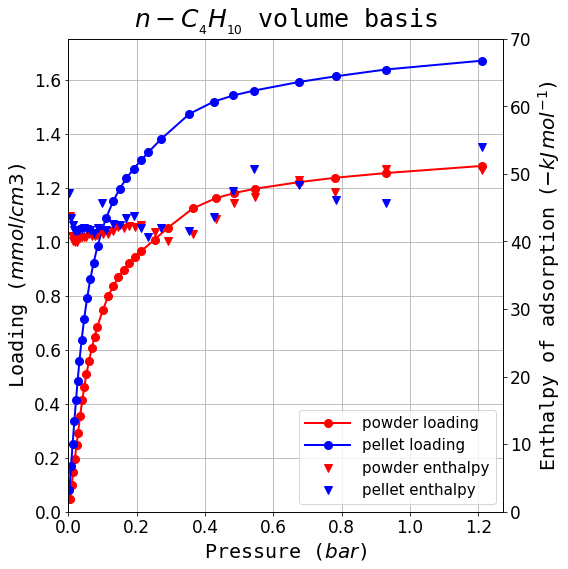
\includegraphics[width=\textwidth]{calo/MIL-100(Fe)/butane-volume-basis-iso}%
        \label{appx:fig:shaping:mil100c4h10volume}
    \end{subfigure}%
    \begin{subfigure}{0.25\textwidth}
        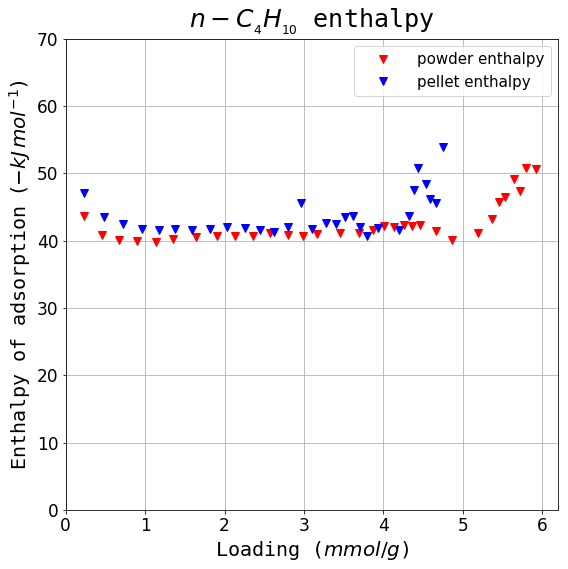
\includegraphics[width=\textwidth]{calo/MIL-100(Fe)/butane-enth}%
        \label{appx:fig:shaping:mil100c4h10enth}
    \end{subfigure}%

    \caption{Complete isotherm and enthalpy dataset for MIL-100(Fe)}%
    \label{appx:fig:shaping:calomil100}
\end{figure}
